% !TeX spellcheck = en_US
\section{Insurances}
\subsection{Efficiency of insurance}
\begin{compactitem}
	\item „Efficiency“ means the right insurance for the right risks for the right price!
	\item One single insurance that fits for all risks doesn’t exist!
	\item Develop with support of an insurance-specialist an „insurance-portfolio“ and validate that portfolio regularly!
\end{compactitem}

\subsection{Basics}
\begin{compactitem}
	\item Who has to bear the damage? Liability insurances vs. „simple“	insurances
	\item What damage? personal injury, material damage or finance damage?
	\item Insured risks (causes): malfunction, manipulations, natural hazards?
	\item Insured risks (objects): third parties, employees, hardware, data-losses, compensation for correct fulfillment, down-time etc.
\end{compactitem}

\subsection{Riskmanagement}
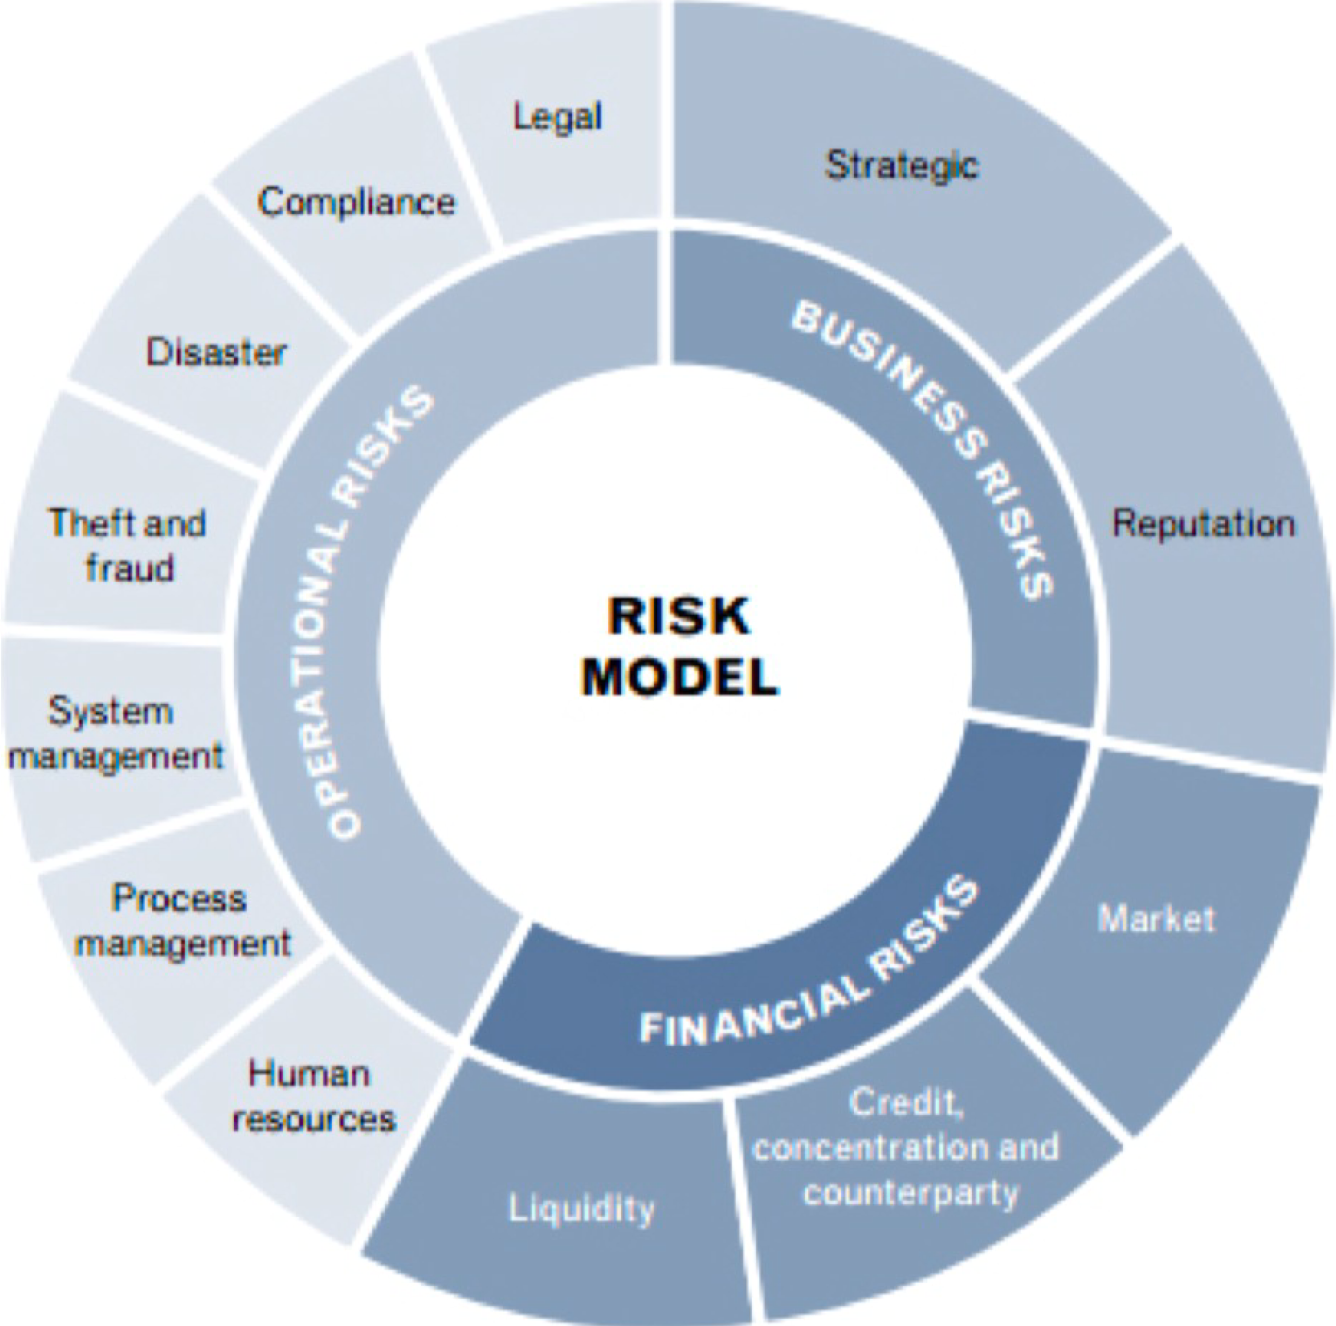
\includegraphics[width=1\linewidth]{images/riskmodel}
\begin{compactitem}
	\item „Climbing, Parachuting, Free-skiing, MX, Diving etc. are not dangerous - dangerous is not to know its risks!“
	\item Remember: RISK = probability of incidence (\%) x potential of damage (CHF)!
	\item Analyse professionally your risks and decide the best strategy to handle the risks!
	\item What’s the best case / worst case scenario? Define clear limits to stop!
	\item „Trust in somebody and you will be disappointed!“
	\item Always watch/control the little things!
	\item Don’t decide accidentally on mood! Make a rational decision based upon clear reasons!
\end{compactitem}

\subsection{Limitations}
\begin{compactitem}
	\item by contractual exclusion
	\item by qualifying period
	\item by the amount of the damage
	\item by direct/indirect damage
\end{compactitem}

\subsection{Legal base}
\subsubsection{Legal limitation - ART. 100 OR}
\begin{compactenum}
	\item Any agreement purporting to exclude liability for unlawful intent	or gross negligence in advance is void.
	\item At the discretion of the court, an advance exclusion of liability for	minor negligence may be deemed void provided the party excluding liability was in the other party’s service at the time the	waiver was made or the liability arises in connection with commercial activities conducted under official license.
	\item the specific provisions governing insurance policies are unaffected.
\end{compactenum}